\FloatBarrier
\begin{figure}
  \centering
  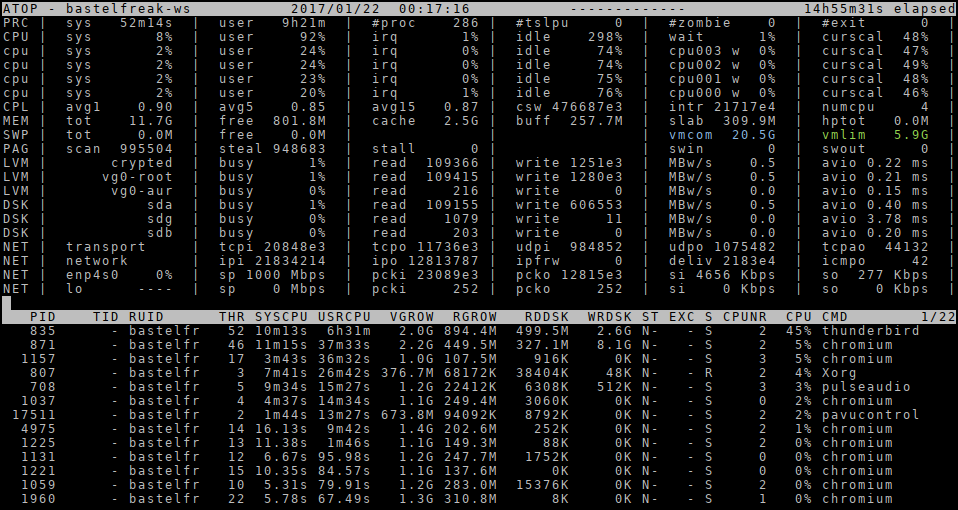
\includegraphics[width=1.0\textwidth]{../figures/atop_1.png}
  \caption{atop mit geringer Systemlast}
\label{figure:atop1}
\end{figure}

\begin{figure}
  \centering
  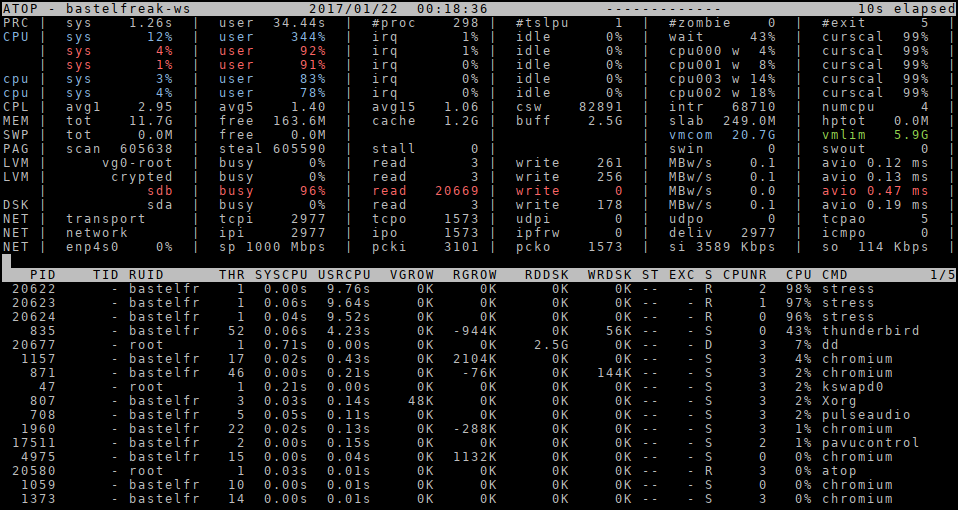
\includegraphics[width=1.0\textwidth]{../figures/atop_2.png}
  \caption{atop mit hoher CPU/Netzwerk Last}
\label{figure:atop2}
\end{figure}

\begin{figure}
  \centering
  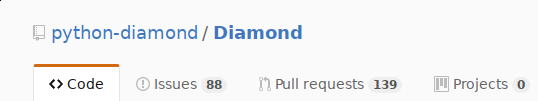
\includegraphics[width=1.0\textwidth]{../figures/diamond.png}
  \caption{Offene PRs und Issues im Diamond Projekt - 22.01.2017}
\label{figure:diamond}
\end{figure}
\FloatBarrier
